\begin{figure}[!t]
	\color{blue}
	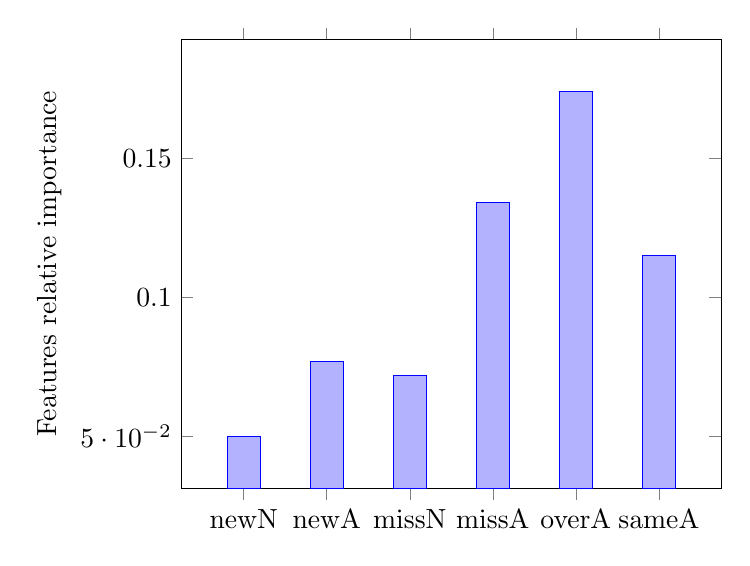
\begin{tikzpicture}
		\begin{axis}[
		ylabel=Features relative importance,
		enlargelimits=0.15,
		legend style={at={(0.5,-0.15)},
			anchor=north,legend columns=-1},
		ybar,
		bar width=12pt,
		 symbolic x coords={newN,newA,missN,missA,overA,sameA}, 
		 xtick=data,
		]
		\addplot 
		coordinates {(newN,0.05) (newA,0.077)
			(missN,0.072) (missA, 0.134) (overA,0.174)
		    (sameA,0.115)};
		
		\end{axis}
	\end{tikzpicture}
	        \caption{
	        	\color{blue}
	        	Relative importance of features from random forest. The features from left to right are 
		\texttt{newN}=number of new coronal holes, 
		\texttt{newA}=image area of new coronal holes,
		\texttt{missN}=number of missing coronal holes,
		\texttt{missA}=image area of missing coronal holes,
		\texttt{overA}=spherical area overestimated by model,
		\texttt{sameA}=spherical area overlap.}
	\label{fig:randomForest_features}
\end{figure}